%! Author = micha
%! Date = 17.03.2021

% Preamble
\documentclass[11pt]{article}

% Packages

\usepackage[margin=1in]{geometry}
\usepackage{listings}
\usepackage{graphicx}
\usepackage{graphics}
\usepackage{hyperref}
\usepackage{algorithmicx}
\usepackage{algpseudocodex}
\usepackage{xcolor}

\colorlet{mygray}{black!30}
\colorlet{mygreen}{green!60!blue}
\colorlet{mymauve}{red!60!blue}

\lstset { %
    backgroundcolor=\color{gray!10},
    basicstyle=\ttfamily,
    columns=fullflexible,
    breakatwhitespace=false,
    breaklines=true,
    captionpos=b,
    commentstyle=\color{mygreen},
    extendedchars=true,
    frame=single,
    keepspaces=true,
    keywordstyle=\color{blue},
    language=c++,
    numbers=none,
    numbersep=5pt,
    numberstyle=\tiny\color{blue},
    rulecolor=\color{mygray},
    showspaces=false,
    showtabs=false,
    stepnumber=5,
    stringstyle=\color{mymauve},
    tabsize=3,
    title=\lstname
}

\geometry{a4paper}
\title{My first document}
\author{Michael Kirsch}
%\date{} % uncomment for no date

% Document
\begin{document}
    \maketitle


    \section{Introduction}
    All set up and ready to go. Lets get some basic concepts.

    \subsection{Textformatting}
    All the things you wanna do emphasis
    \textbf{Bold Formatting}
    \emph{Italics}
    \underline{Michael Underline}
    New para is indented
    \noindent I dont want it indentded


    \section{Oddities}
    Strange things one quoting
    'single' "double"


    \section{List Envs}
    Bulleted List
    \begin{itemize}
        \item Box 1
        \item Box 2
        \item Box 3
    \end{itemize}

    \subsection{Numbered Lists}
    \begin{enumerate}
        \item djwa
        \item dwakd
        \item daw
    \end{enumerate}

    \subsection{Description}
    \begin{description}
        \item [name] Mihcael
        \item[Subject] Stuff
        \item[Grade] A+
    \end{description}


    \section{Nested Stuff}
    \begin{enumerate}
        \item Textformatting
        \item Lists \begin{itemize}
                        \item Bullet
                        \item sorted
                        \item numbered
        \end{itemize}
    \end{enumerate}


    \section{Tables and Floats}
    lets go with tables \bigskip
    padnjiwajdaiodjawio

    \subsection{Tables}
    \vspace{0.5cm}
    \begin{tabular}{|c||c|}
        \hline
        Name  & jdddddddddddddddio \\
        \hline
        Name2 & fajwio             \\
        \hline
        haw   & jdawoi             \\
        \hline
    \end{tabular}

    \subsection{Floats}
    \begin{table}[htbp]
        \caption{Hello World Table}
        \begin{center}
            \begin{tabular}{|c|c|}
                \hline
                Name  & 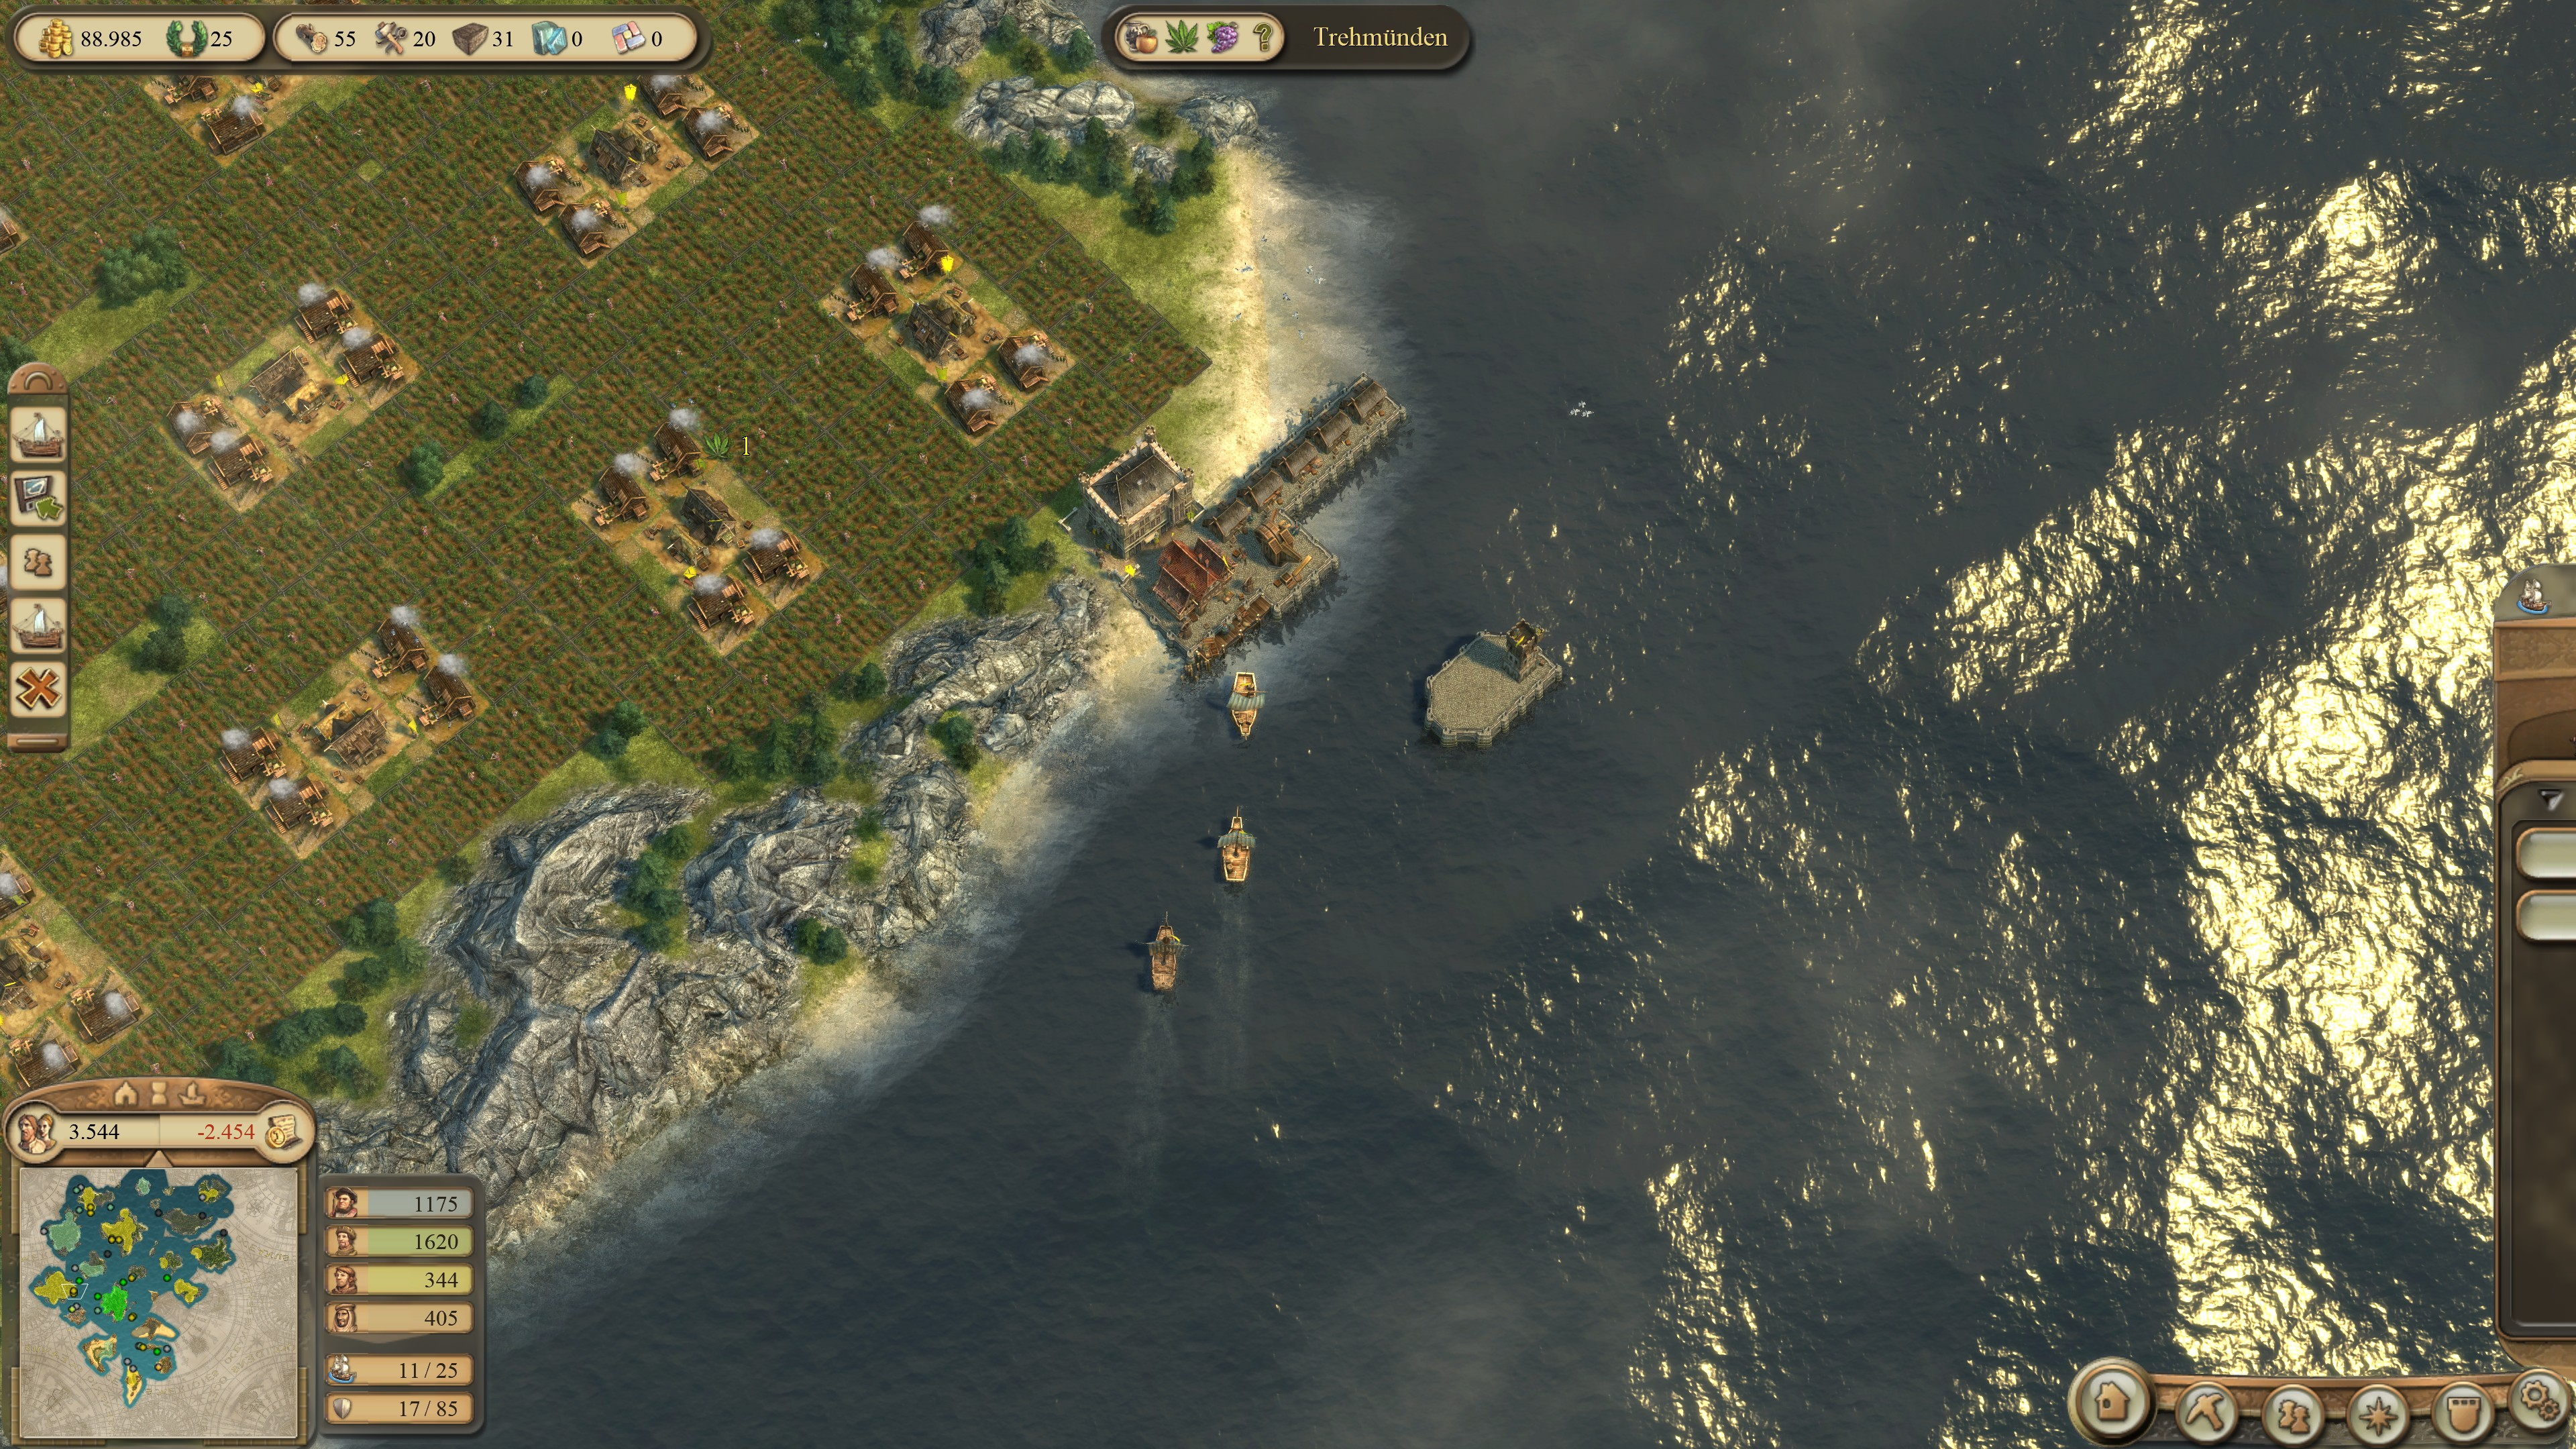
\includegraphics[width=0.7\textwidth]{Anno 1404 - History Edition2021-2-2-1-53-42} \\
                \hline
                Name2 & fajwio                                                                             \\
                \hline
                haw   & jdawoi                                                                             \\
                \hline
            \end{tabular}
        \end{center}
        \label{tab:Important Stuff}
    \end{table}

    \subsection{References}
    Hello badjwidjwiodjawo see Table~\ref{tab:Important Stuff} for more info

% This is comment


    \section{Graphics}
    \begin{equation}
        24*60=1440
        \label{eq:equation}

    \end{equation}


    \begin{figure}[htbp]
        \begin{center}
            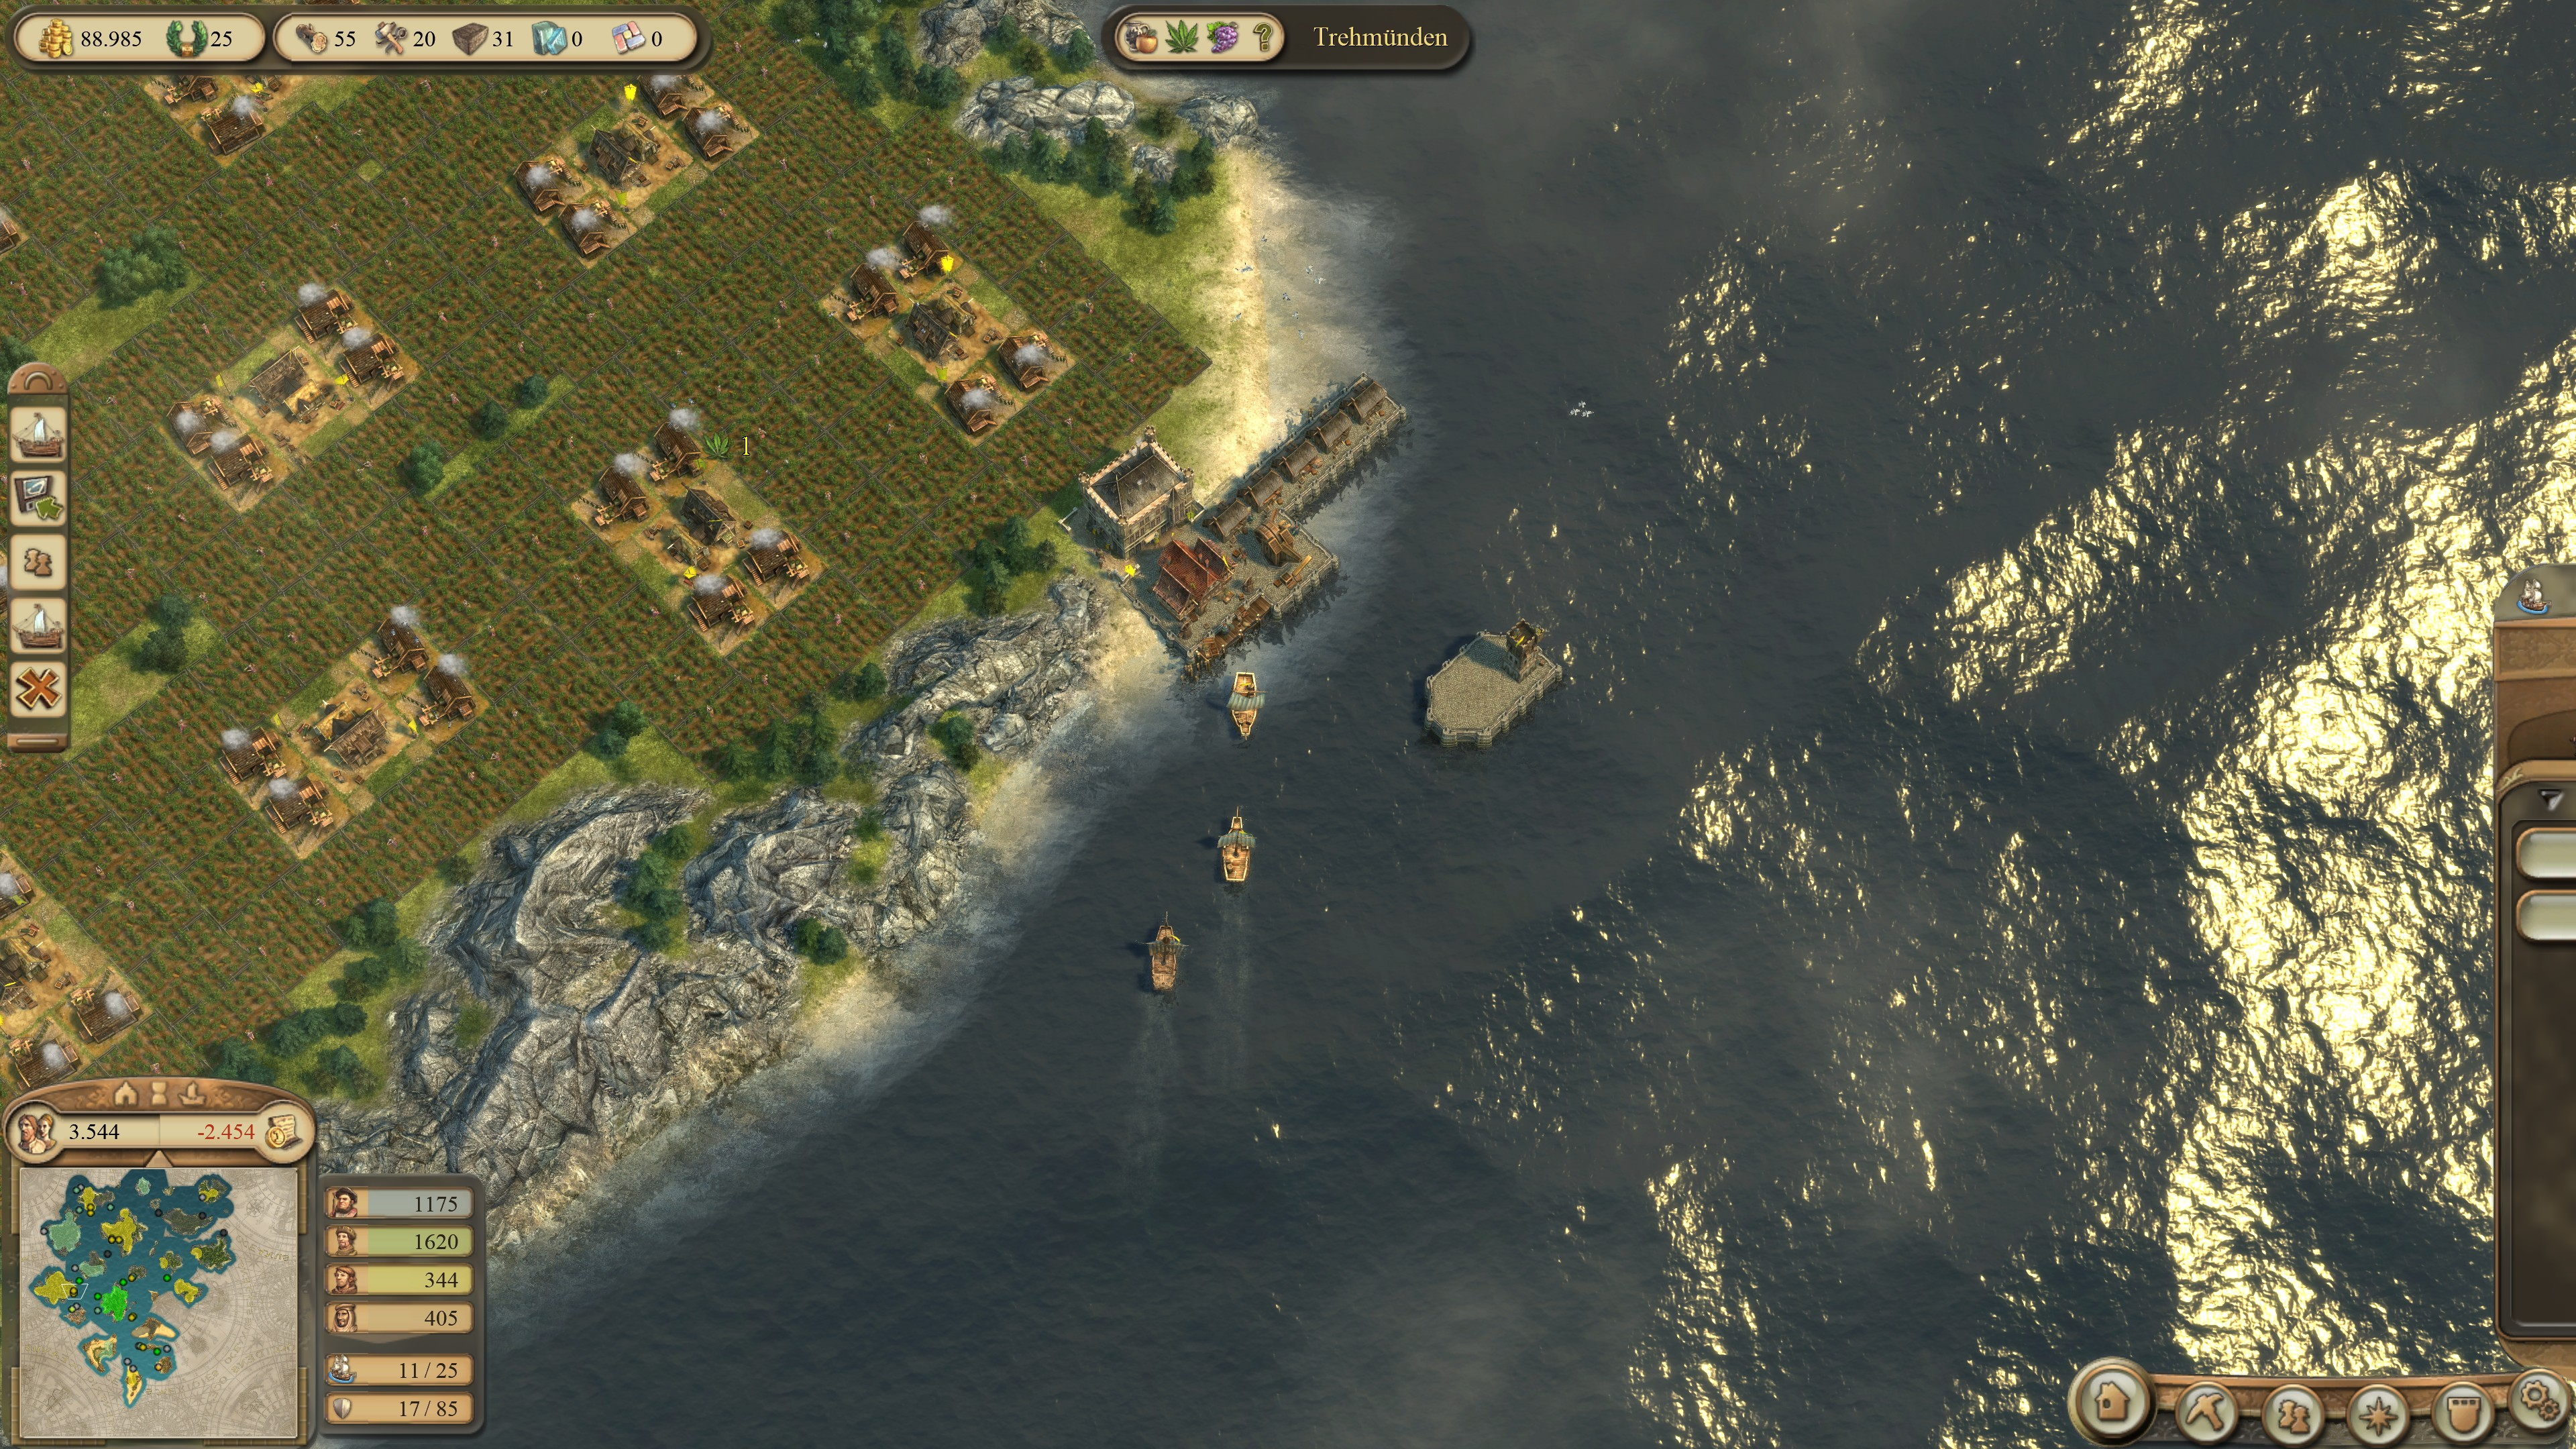
\includegraphics[width=0.7\textwidth]{Anno 1404 - History Edition2021-2-2-1-53-42}
            \caption{This is library}
        \end{center}
        \label{fig:Images}
    \end{figure}

    this is library see \ref{fig:Images}

    $5*4=28$


    ive read a nice book~\cite{two}
    and a good url~\cite{Doe:2009:Online}

    hier referenz~\cite{tollesbuch}


    \section{Algorythms}
    \begin{algorithmic}
        \If{$learned \geg 100$}
            \State $okay \gets true$
            \else
            \While{$not okay$}
                \State repeat
                \State {$okay \gets true$}
            \EndWhile
        \EndIf
    \end{algorithmic}

    \clearpage
    \section{C++ Stuff}
    \begin{lstlisting}[label={lst:lstlisting}]
        #include <tesseract/baseapi.h>
        #include <leptonica/allheaders.h>

        int main()
        {
            char *outText;

            tesseract::TessBaseAPI *api = new tesseract::TessBaseAPI();
            // Initialize tesseract-ocr with English,
            // without specifying tessdata path
            if (api->Init(NULL, "eng")) {
                fprintf(stderr, "Could not initialize tesseract.\n");
                exit(1);
            }

            // Open input image with leptonica library
            Pix *image = pixRead("/usr/src/tesseract/testing/phototest.tif");
            api->SetImage(image);
            // Get OCR result
            outText = api->GetUTF8Text();
            printf("OCR output:\n%s", outText);

            // Destroy used object and release memory
            api->End();
            delete [] outText;
            pixDestroy(&image);

            return 0;
        }
    \end{lstlisting}


    \bibliographystyle{plain}
    \bibliography{first_example}
\end{document}